\chapter{Overview of the relevant techniques and graph learning architectures}
\label{chapter3}
\thispagestyle{plain}

\section{Surface networks}
In math by \textit{surface} is intended a function f of one or more variables. In geography one is usually interested in those functions for which two of the independent variables denote location in a geographic domain; that is, functions f(u,v) where (u,v) denotes a point within a geographic
coordinate system. A topographic surface in which altitude is a function of position is a convenient prototype.  \textit{Surface Networks} are an abstraction of the 2-dimensional surfaces by storing only the most important (also called fundamental, critical or surface-specific) points and lines in the surfaces.

Surface networks allow to abstract the Earth's surface and store its fundamental properties. These networks can be represented as graphs whose nodes and edges are extracted from the Earth's shape by finding its critical points. In math, the critical points can be  classified as maxima (or peaks), minima (or pits) and saddles (or passes).
If we define a surface's function \(y = f(\textbf{x})\), then we can think at the maxima as those points whose value of the function \(f(\textbf{x})\) is the highest compared to their neighbours. We can distinguish between local maxima and global maxima; local maxima are the points whose function value is the largest within a given range, while a global maximum is the point that has the highest value for the entire domain of the function. Accordingly, local minima are those points whose value of the function is the smallest within a given range, while the global minimum is the smallest for the entire function. Finally saddles are those points that are connected to two local (global) maxima and to two local (global) minima. The connection to the local maxima is given by following the two most steepest ascent paths starting from the saddle and reaching the maxima, while the local minima are reached by following the two most steepest descend paths.
Examples of critical points for a 3-dimension surface defined by a function \(z = f(x,y)\), such as the Earth, can be seen in Figure \ref{fig:critical_points}.

\begin{figure} 
\centering
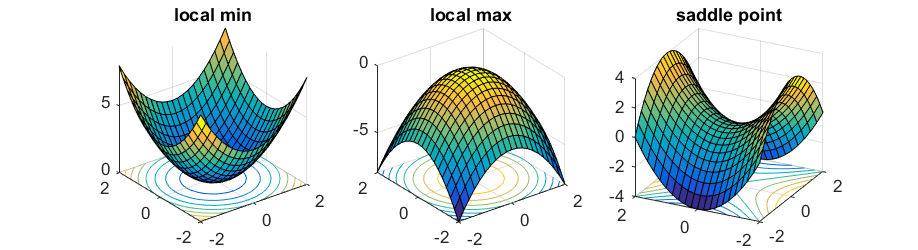
\includegraphics[width=12cm]{minmaxsaddle.png}
\caption{Critical Points}
Figure illustrating the 3 types of critical points of a continuous surface.
\label{fig:critical_points}
\end{figure}

Surface networks capture the topological relations between the critical points of a continuous surface. In a surface network, every saddle is connected, at least, to two maxima and to two minima. The paths with the steepest ascents starting from a saddle connect it to the maxima, while the paths with the steepest descents connect it to the minima. The resulting graph of critical points and critical lines connecting them is termed \textit{surface network} (Pfaltz 1976) \cite{surface_networks_rana}. An example of surface network for a portion of the Latschur Mountains in Western Carinthia, Austria can be seen in Figure \ref{fig:surface_network}. Surface networks represent special types of graphs with the vertexes set consisting of the critical points and the edges set consisting of the critical lines.

\begin{figure} 
\centering
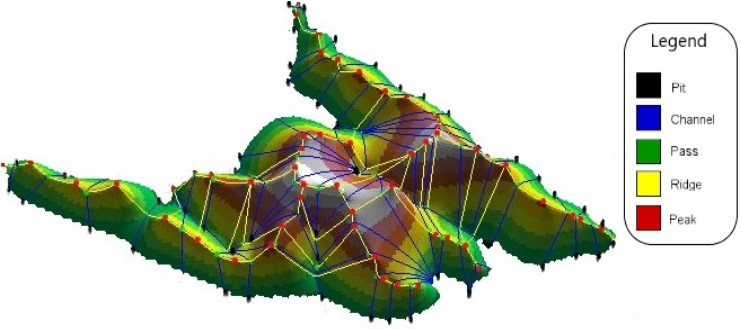
\includegraphics[width=13cm]{Surface_Networks.jpg}
\caption{Surface Network}
Figure illustrating a surface network. The critical points are evidenced with red for peaks (maxima), black for pits (minima) and green for passes (saddles). In morphology the connections between saddles and maxima points are called ridges and here represented with a yellow line, while the connections between saddles and minima are called channels, here showed with a blue line. Image taken from the work of Sanjay Rana and Jeremy Morley in \cite{surface_networks_rana}.
\label{fig:surface_network}
\end{figure}

\subsection{Building Surface Networks from Raster Data}
Contemporary Geographical Information Systems (GISs) for representing Earth's surface are using as a main data structure the so called \textit{digital elevation models (DEMs)}. A DEM can be defined as a raster (a grid of squares, also known as a heightmap when representing elevation) or as a vector-based triangular irregular network (TIN). We used as terrain representations mainly the rasters, i.e. matrices  containing the elevations for the areas they were representing. Different sources for the DEMs can be cited, such as Laser Imaging Detection and Ranging (LiDAR) or Shuttle Radar Topography Mission (SRTM) missions \cite{Farr2007RGP}. By using DEMs, the critical points and their connections cannot be evaluated like in classical differential topology where we analyze the derivatives of the surface. Instead, DEMs are an approximation of surfaces and they are not continuous; indeed each cell of the matrix represent a different elevation, and moving from a cell to another leads to discontinuous changes. An example of a small portion of a DEM containing elevations can be seen in Figure \ref{fig:dem_raster}. 
\begin{figure} 
\centering
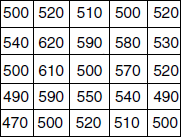
\includegraphics[width=5cm]{dem_raster.png}
\caption{DEM raster}
Figure illustrating a portion of DEM raster containing elevations expressed in meters.
\label{fig:dem_raster}
\end{figure}

Traditional methods for finding the critical points and their connections involve considering for each cell its eight direct neighbours, and based on the comparison among this neighbourhood it can be classified as : peak, pit, pass, ridge, channel, plane. A cell is considered a maximum (peak) if it is the highest one among its 8 neighbours, while it is a minimum (pit) if it is the lowest one. A cell is a saddle (or pass) if it is the highest point considering the direction given by two of its neighbours that are not adjacent among them and it is the lowest point considering another direction given by other two non adjacent cells of its neighbours. An area composed by nine (or more) cells where all have the same elevation is a plane. Finally, the channels are composed by a sequence of cells surrounded by higher ones, while the ridges are a sequence of higher cells compared to the neighbours. These six basic morphometric classes can be identified with the eight-neighbours method, and an example can be seen in Figure \ref{fig:six_morphometric}.

The method of Shigeo Takahashi  \cite{extracting_surface_topology} for the creation of surface networks suggests that features like critical points and their connections come from the theory of differential topology and they should satisfy some topological formulas. The most important one is the \textit{Euler-Poincarè formula} which states that the total number of critical points for a surface satisfies this property: \#maxima - \#saddles + \#pits = 2. Here \# means "number of". As said in \cite{extracting_surface_topology} the eight direct neighbours method finds a set of critical points which does not satisfy this rule. Shigeo Takahashi proposed an algorithm for extracting critical points that preserves the validity of the Euler-Poincarè formula. The proposed method is based on the \textit{Delaunay triangulation} for defining the neighborhood of a cell without incurring in unwanted critical points which happens with standard methods like the one proposed by Peucker and Douglas in \cite{peackerAndDouglas}. The Delaunay triangulation is a subdivision of a set of points into a non-overlapping set of triangles, such that no point is inside the circumcircle of any triangle. In practice, such triangulations tend to avoid triangles with small angles. In the case study of DEMs the triangulation is defining for each cell of the matrix which of the adjacent cells is a neighbour, i.e. not all the adjacent cells are considered anymore neighbours. As we can see in Figure \ref{fig:delaunay_triangulation} each cell is surrounded by other eight cells but there is not a connection with all of them.
\begin{figure} 
\centering
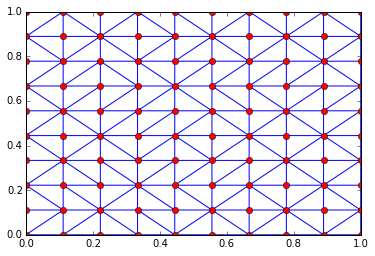
\includegraphics[width=10cm]{delaunay_figure.png}
\caption{Delaunay Triangulation}
Figure illustrating a portion of DEM and the Delaunay triangulation. The red dots represents the cells of the raster while the blu lines how the triangulation is setting the neighbours of each cell.
\label{fig:delaunay_triangulation}
\end{figure}
Instead of extracting critical points directly from DEMs, Wood suggested in \cite{wood_book} a method for specifying bi-variate quadratic surface patches at raster points. These surface patches make possible to identify the directions of steepest descent and ascent and allowing then to identify the critical points and critical lines. The great benefit of the bi-variate quadratic surfaces is that they can be fitted to windows of any size enabling to perform the analysis on a desired level of scale. However, this approach does not guarantee consistency of the extracted network. Still based on the idea of interpolating surfaces B. Schneider proposes in \cite{Schneider} a simpler bilinear interpolation scheme allowing a less flexible but more rigorous method in terms of continuity. These researches sometimes refer to the surface networks as \textit{metric} or \textit{weighted} surface networks. These versions assign a weight to the edges of the graph; the most common kind of weight is the difference of elevation between the two nodes considered.

\section{ Machine Learning Techniques}
\subsection{Logistic Regression}\label{sec:logistic_regression}
\subsection{Node2Vec}
\subsection{GraphSAGE}

...others...